\colorlet{punct}{red!50!black}
\definecolor{background}{HTML}{F3F6FF}
\definecolor{delim}{RGB}{20,105,176}
\colorlet{numb}{magenta!50!black}

\lstdefinelanguage{json}{
	basicstyle=\tiny\ttfamily,
	numberstyle=\scriptsize,
	stepnumber=1,
	numbersep=4pt,
	showstringspaces=false,
	breaklines=true,
	frame=lines,
	backgroundcolor=\color{background},
	literate=
	*{:}{{{\color{punct}{:}}}}{1}
	{,}{{{\color{punct}{,}}}}{1}
	{\{}{{{\color{delim}{\{}}}}{1}
	{\}}{{{\color{delim}{\}}}}}{1}
	{[}{{{\color{delim}{[}}}}{1}
	{]}{{{\color{delim}{]}}}}{1},
}


\chapter{Sincronización de Resultados}

\label{chapA:rest-api}

En este anexo, se proporcionan detalles adicionales los servicios RESP para realizar, incluyendo ejemplos y relación entre los recursos.

El servicio se comprende de dos recursos \textit{Collaborativefeature} y \textit{Collaborativesession}, el primero de estos representa la colección de los 15 feature calculados de una ventana de tiempo, y por otro lado la session de una actividad realizada por el individuo, la cual incluye una lista de features, como se esquematiza en la siguiente figura \ref{fig:der} .

\begin{figure}[!htbp]
	\centering
	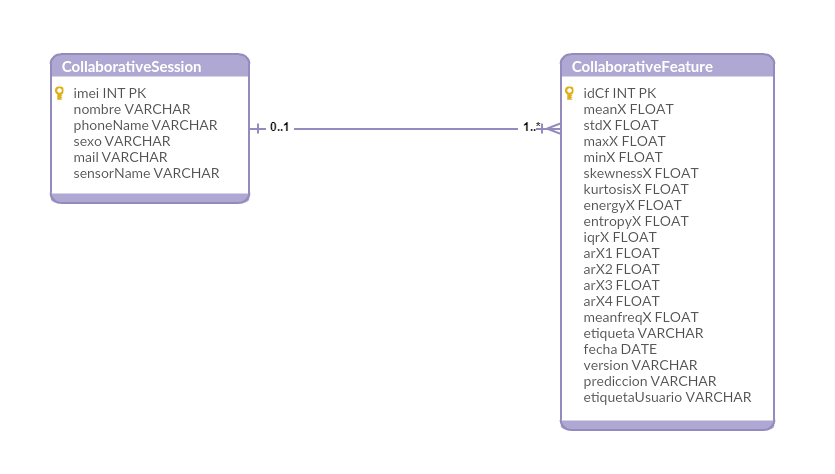
\includegraphics[width=0.7\linewidth]{anexos/der}
	\caption[Modelo de Datos]{\label{fig:der}Modelo de Datos}
\end{figure}

Los datos de la API publicada son las siguientes:

\textit{\textbf{http://[URL:PUERTO]/[CONTEXTO]/[RECURSO]/}}

Estando publicadas para las pruebas:

\begin{itemize}
	\item URL:PUERTO: ec2-52-27-63-54.us-west-2.compute.amazonaws.com:8080
	\item Contexto: ARrecolector
\end{itemize}



\section{Recurso CollaborativeSession}

\subsection{Creación de Objeto - POST}

Para crear una session de entrenamiento, se utiliza el metodo POST al recurso \textit{ARrecolector/webresources/com.fpuna.entities.collaborativesession/} con el siguiente ejemplo del request JSON \ref{lst:POST}:

\begin{lstlisting}[language=json,firstnumber=1,label={lst:POST}]
{
  "imei": "ea3fb543-fec3-3bb5-be2b-006082c66b33",
  "phoneName": "Samsung SM-G925I",
  "sexo": "m",
  "nombre": "joaquinlima@gmail.com",
  "edad": "35",
  "sensorName": "MPU6500 Acceleration Sensor Invensense",
  "collaborativefeatureList": [
     {
       "arX1": 0,
       "arX2": 0,
       "arX3": 0,
       "arX4": 0,
       "energyX": 0,
       "entropyX": 0,
       "etiqueta": "WALKING",
       "fecha": "2015-12-23T02:33:24-02:00",
       "idCf": 3,
       "iqrX": 0,
       "kurtosisX": 0,
       "maxX": 0,
       "meanX": 0,
       "meanfreqX": 0,
       "minX": 0,
       "skewnessX": 0,
       "stdX": 0,
       "version": "1.0",
       "prediccion": "S",
       "etiquetaUsuario": "STILL"
     },{ 
	     -- More feature -- 
     }  
  ]
}
\end{lstlisting}

\subsection{Obtención de Recurso - GET}

Para recuperar una session de entrenamiento, se utiliza el metodo GET al recurso \textit{ARrecolector/webresources/com.fpuna.entities.collaborativesession/[IDENTIFICADOR]}, siendo el identificador el imei de la session. Obteniendo un response de la siguiente manera:

\begin{lstlisting}[language=json,firstnumber=1,label={lst:GET}]
{
  "imei": "ea3fb543-fec3-3bb5-be2b-006082c66b33",
  "phoneName": "Samsung SM-G925I",
  "sexo": "m",
  "nombre": "joaquinlima@gmail.com",
  "edad": "35",
  "sensorName": "MPU6500 Acceleration Sensor Invensense",
  "collaborativefeatureList": [
    {
      "arX1": 2.24001,
      "arX2": -1.56002,
      "arX3": 0.319989,
      "arX4": -0.00000347302,
      "energyX": 95.5371,
      "entropyX": 6.9375,
      "idCf": 1439,
      "iqrX": 0.277481,
      "kurtosisX": 0.0359763,
      "maxX": 10.3113,
      "meanX": 9.77168,
      "meanfreqX": 9.81451,
      "minX": 9.2704,
      "skewnessX": 0.0880117,
      "stdX": 0.227583,
      "etiqueta": "WALKING",
      "fecha": "2015-12-23T02:33:24-02:00",
      "version": "1.0",
      "prediccion": "S",
      "etiquetaUsuario": "WALKING"
    },{ 
	     -- More feature -- 
    }
  ]
}
\end{lstlisting}

\subsection{Modificación de Recurso - PUT}

Para modificar una session de entrenamiento, se utiliza el metodo PUT al recurso \textit{ARrecolector/webresources/com.fpuna.entities.collaborativesession/[IDENTIFICADOR]}, siendo el identificador el imei de la session a modificar. Utilizando un request JSON de la siguiente manera:

\begin{lstlisting}[language=json,firstnumber=1,label={lst:PUT}]
{
  "imei": "ea3fb543-fec3-3bb5-be2b-006082c66b33",
  "phoneName": "Samsung SM-G925I",
  "sexo": "m",
  "nombre": "joaquinlimaMolinari@gmail.com",
  "edad": "35",
  "sensorName": "MPU6500 Acceleration Sensor Invensense",
  "collaborativefeatureList": [
    {
      "arX1": 2.24001,
      "arX2": -1.56002,
      "arX3": 0.319989,
      "arX4": -0.00000347302,
      "energyX": 95.5371,
      "entropyX": 6.9375,
      "idCf": 1439,
      "iqrX": 0.277481,
      "kurtosisX": 0.0359763,
      "maxX": 10.3113,
      "meanX": 9.77168,
      "meanfreqX": 9.81451,
      "minX": 9.2704,
      "skewnessX": 0.0880117,
      "stdX": 0.227583,
      "etiqueta": "WALKING",
      "fecha": "2015-12-23T02:33:24-02:00",
      "version": "1.0",
      "prediccion": "S",
      "etiquetaUsuario": "WALKING"
    },{ 
      -- More feature -- 
    }  
  ]
}
\end{lstlisting}

\subsection{Eliminación - DELETE}

Para eliminar una session de entrenamiento, se utiliza el metodo DELETE al recurso \textit{ARrecolector/webresources/com.fpuna.entities.collaborativesession/[IDENTIFICADOR]}, siendo el identificador, el imei de la session que se desea eliminar. 

\section{Recurso CollaborativeFeature}

De la misma manera que el recurso anterior, están implementados todos los métodos CRUD, con POST, GET, PUT, DELETE, permitiendo el acceso de manera completa a todos los recursos colaborativos.